\ifx\pdfminorversion\undefined\else\pdfminorversion=4\fi
\documentclass[aspectratio=43,t]{beamer}
%\documentclass[aspectratio=43,t,handout]{beamer}

% English version FAU Logo
%\usepackage[english]{babel}
% German version FAU Logo
\usepackage[ngerman]{babel}

\usepackage[utf8]{inputenc}
\usepackage[T1]{fontenc}
\usepackage{amsmath,amssymb}
\usepackage{graphicx}
\usepackage{minted}
\usepackage{subcaption}
\usepackage[backend=biber,sorting=none,doi=true,style=ieee]{biblatex}

\setminted{fontsize=\scriptsize}
% Options:
%  - inst:      Institute
%                 med:      MedFak FAU theme
%                 nat:      NatFak FAU theme
%                 phil:     PhilFak FAU theme
%                 rw:       RWFak FAU theme
%                 rw-jura:  RWFak FB Jura FAU theme
%                 rw-wiso:  RWFak FB WISO FAU theme
%                 tf:       TechFak FAU theme
%                 tf-hscd:  TechFak Co-Design FAU theme
%  - image:     Cover image on title page
%  - plain:     Plain title page
%  - longtitle: Title page layout for long title
\usetheme[%
  inst=tf-hscd,%
  longtitle%
]{fau}

% Enable semi-transparent animation preview
\setbeamercovered{transparent}

\defbibheading{bibliography}{}
\addbibresource[label=primary]{references.bib}
\nocite{*}


% Title, authors, and date
\title[Backtracking]{Backtracking}
\subtitle{Ausgewählte Kapitel aus "The Art of Computer Programming"}
\author[Bastian Kauschke]{Bastian Kauschke}
% English version
%\institute[Hardware/Software Co-Design]{Hardware/Software Co-Design, Friedrich-Alexander University Erlangen-Nürnberg}
% German version
\institute[Hardware-Software-Co-Design]{Hardware-Software-Co-Design, Friedrich-Alexander-Universität Erlangen-Nürnberg}
\date{\today}
% Set additional logo (overwrites FAU seal)
%\logo{
\includegraphics[width=.15\textwidth]{themefau/art/tf/hscd/codesign.pdf}}


\begin{document}
  % Title
  \maketitle

  { % Outline
    \setbeamertemplate{footline}{}
    \begin{frame}[noframenumbering]{Outline}
      \tableofcontents
    \end{frame}
  }

  % Body
  \section{Einführung}
  \begin{frame}{Anwendungsbereich}
    Sequenzen $x_{1}, x_{2}, x_{3} \dots x_{n}$ für welche die Bedingung $P_{n}(x_{1}, x_{2}, x_{3} \dots x_{n})$ gilt.\\
    \ \\ 
    $P$ hat dabei folgende Eigenschaften: \pause
    \begin{itemize}
      \item $P_{l}(x_{1}, x_{2}, x_{3} \dots x_{l})$ gilt nur, wenn $P_{l-1}(x_{1}, x_{2}, x_{3} \dots x_{l-1})$ gilt \pause
      \item wenn $P_{l}(x_{1}, x_{2}, x_{3} \dots x_{l})$ gilt, ist $P_{l+1}(x_{1}, x_{2}, x_{3} \dots x_{l+1})$ einfach zu testen \pause
      \item $P_{0}()$ gilt immer
    \end{itemize}
  \end{frame}

  \begin{frame}[fragile]{Algorithmus}
    \begin{minted}{rust}
/// A required set of methods needed for the generic backtracking algorithms.
pub trait Sequence {
    type Step;
    type Steps: IntoIterator<Item = Self::Step>;

    /// Checks if this sequence satisfy its condition.
    ///
    /// This function can assume that the  parent of `self` satisfied this condition.
    fn satisfies_condition(&self) -> bool;

    /// generates all possible next steps at this current state.
    fn next_steps(&self) -> Self::Steps;

    /// applies a `step` to `self`, returning the resulting sequence.
    ///
    /// this function will only be called if `self.satisfies_condition() == true`.
    fn apply_step(&self, step: Self::Step) -> Self;
}

      \end{minted}
    \end{frame}
    \begin{frame}[fragile]{Algorithmus}
      \begin{minted}{rust}
pub fn b<T: Sequence>(initial: T, n: usize) -> Vec<T> {
    let mut results = Vec::new();
    let mut states = Vec::new();
    let steps = initial.next_steps().into_iter();
    states.push((initial, steps));

    while let Some((state, steps)) = states.last_mut() {
        if let Some(step) = steps.next() {
            let next_state = state.apply_step(step);
            if next_state.satisfies_condition() {
                if states.len() < n {
                    let next_steps = next_state.next_steps().into_iter();
                    states.push((next_state, next_steps));
                } else {
                    results.push(next_state);
                }
            }
        } else {
            states.pop();
        }
    }
    results
}
    \end{minted}
  \end{frame}
  \section{n Queens}
    \begin{frame}{Damenproblem}
      Wie viele Möglichkeiten gibt es $n$ Damen auf einem $n * n$ Schachbrett aufzustellen, dass sich keine zwei Damen schlagen können.
      Also keine 2 Damen in der selben Zeile, Reihe oder Diagonalen stehen.
      \begin{figure}[h!]
        \centering
        \begin{subfigure}{0.4\linewidth}
          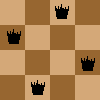
\includegraphics[width=\linewidth]{../img/queensRight.png}
          \caption{Richtig}
        \end{subfigure}
        \begin{subfigure}{0.4\linewidth}
          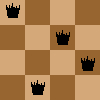
\includegraphics[width=\linewidth]{../img/queensWrong.png}
          \caption{Falsch}
        \end{subfigure}
        \label{n4}
      \end{figure}

    \end{frame}
    %\pause

    %\begin{block}{Numbered List of Items}
    %%  \begin{enumerate}
     %   \item<2-> one
     %   \item<3-> two
     %   \item<4-> three
     %   \item<5-> \dots
     % \end{enumerate}
    %\end{block}

  \section{Listings}
  \begin{frame}[fragile]{Listings}
    empty
  \end{frame}

  { % Questions?
    \setbeamertemplate{footline}{}
    \begin{frame}[c,noframenumbering]
      \begin{center}
        Thanks for listening.\\
        {\bf Any questions?}
      \end{center}
    \end{frame}

    % References
    \section*{References}
    \begin{frame}[allowframebreaks,noframenumbering]{References}
      \printbibliography
    \end{frame}
  }
\end{document}

